\section{Fault Modeling and the Safety Annex}
\label{sec:fault_modeling}

\subsection{Features Needed for Fault Modeling}
It is assumed that an AADL model of the nominal system specifies the hardware, software, and mechanical components of the system and their interconnections. This model is annotated with behavioral contracts using the AGREE annex~\cite{NFM2012:CoGaMiWhLaLu}. The nominal model behavioral requirements are verified using inductive model checking through AGREE~\cite{2017arXiv171201222G}. At this point, the fault modelling can commence. 

When conducting the safety assessment and examining the individual subcomponents of a system, the faults and failure modes must be determined. A fault is the manifestation of an error that may lead to failure in a given component~\cite{SAE:ARP4754A}. For example, a fault in a valve may be that it is stuck closed. If this fault is active, it may cause a failure to occur. If there is no command to provide outgoing pressure, then this active fault will not cause a failure of the component to perform as intended. On the other hand, if there is such a command to provide pressure, this fault will cause failure of the valve component. The failure mode in this case is that there is a command to provide outgoing pressure, but an active fault on the valve causes it to be stuck closed. We use {\em fault} as the generic modeling keyword throughout the AADL model hierarchy and follow the definitions of these terms (error, failure, fault) throughout this description.

Many of these modes can be determined through domain knowledge and other modes are specified through the manufacturer of a given mechanical or digital component. Once the faults and failure modes are determined, the safety engineer must determine the consequence of this component failure on connected components, components that are physically located nearby, and on the system as a whole. Given that many safety critical systems are quite complex, this propagation process can be error prone and time consuming.

In the following subsections, we walk through examples of component failure modes to illustrate how a safety engineer can use the Safety Annex to model these modes and see how an active fault may or may not cause failure of a component.

In the AADL system model and the AGREE behavioral model, we have the component structures and behaviors (properties) defined for the system subcomponents. Assuming that the nominal model holds (in the absence of errors, the system behavior is correct), it is of interest to see how the manifestation of errors impacts the overall system functionality. To determine this information, a safety engineer must determine what possible errors could be present in the given components of the system and if the manifestation of these errors will cause a systems functionality to be erroneous. Many of these component errors originate in software and when these errors manifest in real life, they are propagated implicitly through the system. For example, when a valve is stuck closed the effects of this component failure can be seen through the behavioral contracts and need not be explicitly modelled. But this does not cover all possible failure types. As an example, assume there are colocated pipes and one bursts. Given the nature of the failure, this could affect the behavior of the colocated pipe and thus must be explicitly propagated. In the system model, there are no connections between these components, only in the physical world are they related. For this reason, a safety analyst must be able to define explicit propagation as well as implicit.  

In the following subsections, we describe the modelling process for these failure modes using the WBS as a reference model. 

\subsection{Implicit (Behavioral) Failure Propagation}
When using the Safety Annex to model behavioral failure propagation, a \textit{fault} is attached to a component, which when active will change the output of said component. This faulty value on the output may or may not violate the contracts of the component and it may or may not violate the assumptions of the destination component. These details are seen through the output of the model checker when the safety analysis is run on the fault model. Examples of such faults include valves being stuck open or closed, output of a software component being nondeterministic, or power being cut off. These component types range from mechanical to digital, but for this section we focus on a digital component in the WBS, a sensor on the pedal component. 

The purpose of the safety analysis process is to guarantee that certain top level safety properties of the system hold with certain reliability in the presence of faults. In the WBS, there are a number of safety properties of interest and we focus on one: Inadvertant braking. As described in Section~\ref{subsubsec:wbs:behavior}, one of the components important to the property \textit{Inadvertant braking}, is the pedal. When the mechanical pedal is pressed, a sensor reads this information and passes an electronic signal to the BSCU which then proceeds in commanding hydraulic pressure to the wheels. 

\begin{figure}[h!]
	\hspace*{-2cm}
	\vspace{-0.4in} 
	\begin{center}
		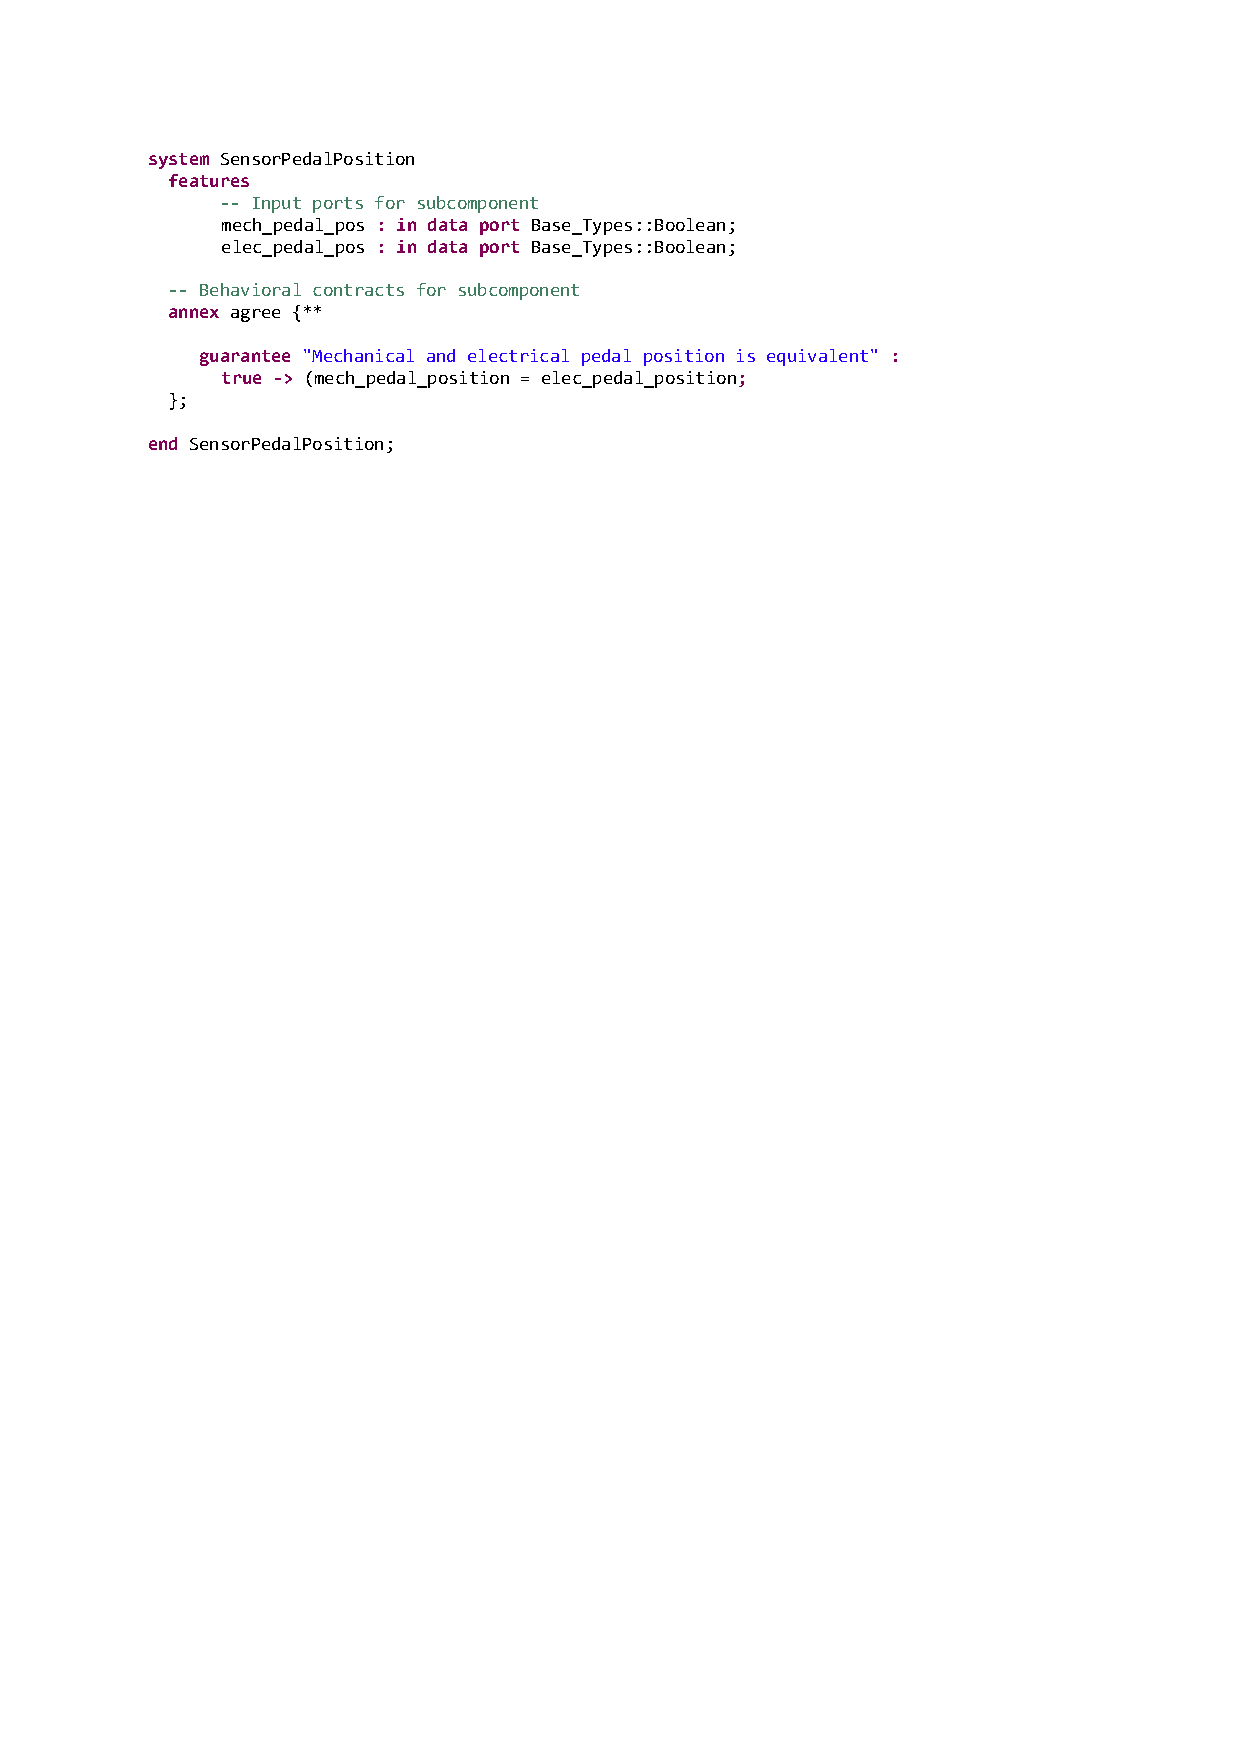
\includegraphics[trim=0 640 -10 70,clip,width=1.5\dimexpr\textwidth-2cm\relax]{images/system_sensor.pdf}
		\caption{An AADL System Type: The Pedal Sensor}
		\label{fig:sensor}
	\end{center}
	\vspace{-0.3in}
\end{figure}

In Figure~\ref{fig:sensor}, the AADL system component is shown with a contract on the output of this component. The sensor has only one input: the mechanical pedal position and one output: the electrical pedal position. The property that governs the behavior of the component is that the mechanical position should always equal the electronic position. This is an example of the nominal system model in AADL with behaviors defined in AGREE. 

\begin{figure}[h!]
	\hspace*{-2cm}
	%\vspace{-0.4in} 
	\begin{center}
		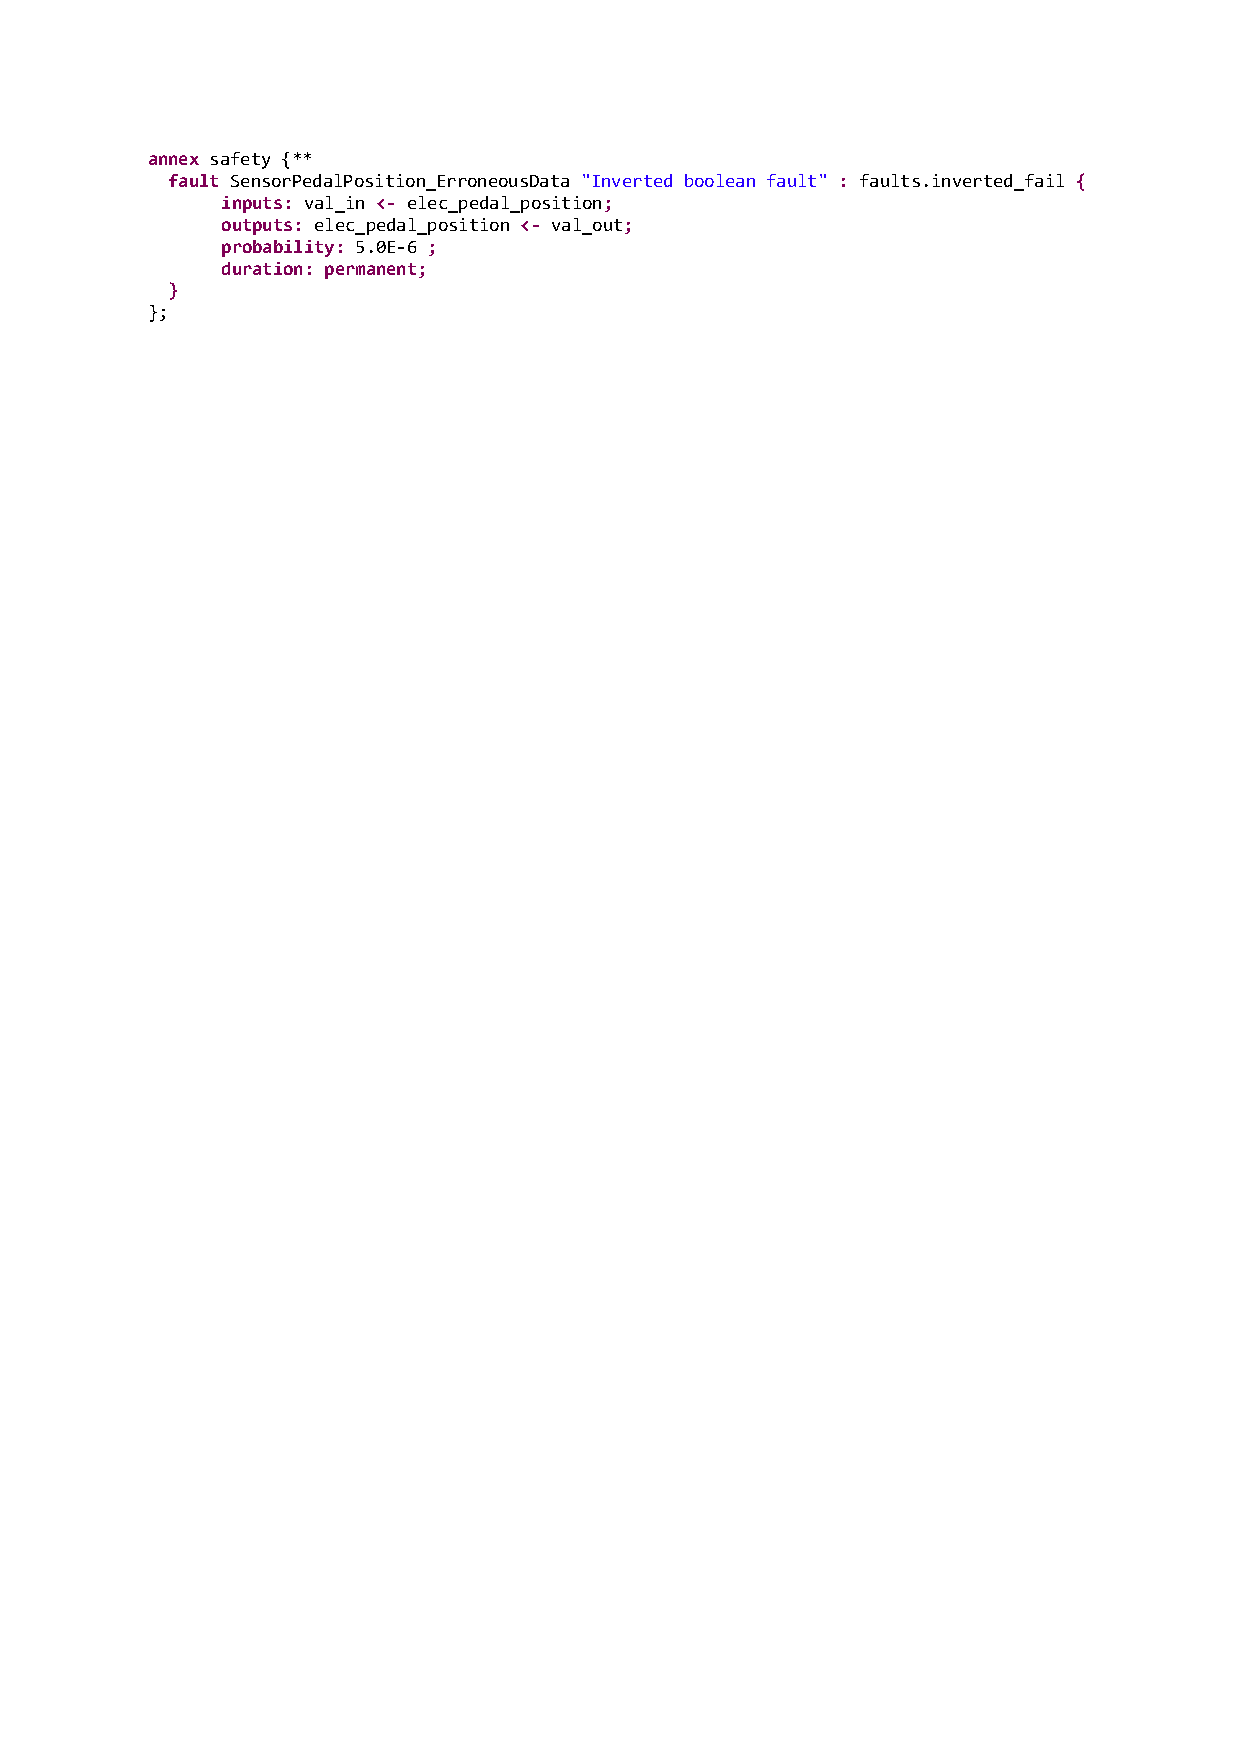
\includegraphics[trim=0 690 -10 70,clip,width=1.5\dimexpr\textwidth-2cm\relax]{images/safetyannex_sensorfault.pdf}
		\caption{The Safety Annex for the Pedal Sensor}
		\label{fig:sensorFault}
	\end{center}
	\vspace{-0.3in}
\end{figure}

This sensor has a known failure which can invert the signal read and pass along an incorrect value. This fault which causes this failure is triggered with probability $5.0e-6$. In Figure~\ref{fig:sensorFault}, the Safety Annex definition for this fault is shown. The faults are defined using a library of fault nodes (in this case, \textit{inverted\_fail}) and when the fault is triggered, the output of the component (\textit{elec\_pedal\_position}) is converted into its failure value (\textit{val\_out}). 

When this particular fault is active in the system, we can run the analysis to see how it propagates through the system. The classification of the top level safety property is catastrophic and carries a probability threshold of $1.0e-9$. Upon running the fault analysis in the toolset, a counterexample is provided for this top level property given the fault definition provided in Figure~\ref{fig:sensorFault}. Since the probability of this fault occuring on the sensor is higher than that of the top level property, it is of interest. 

Through the counterexample display we can trace the behavior of the system through the active faults as well as the violated contracts. The mechanical pedal is not pressed, but this failure causes the sensor subcomponent to report to the BSCU that it was pressed. The active BSCU channel uses this value in order to command braking, determine validity of the channel and control the antiskid behavior of the aircraft. The BSCU carries on with its normal behavior assuming that the pedal was pressed and the state of the system is as follows: braking is not commanded and power is supplied throughout the system. The ground is moving, there is braking force at the wheels, and the wheel is rolling. Taken together this clearly disproves the top level contract that inadvertant braking at a given wheel does not occur. Thus the safety analyst of this system can recognize that some set of precautions such as redundancy are required for the pedal sensor component. 

\subsection{Explicit Failure Propagation} 

As described in Section~\ref{subsec:comparison_with_EMV2}, explicit fault propagation is something that currently exists in EMV2 for AADL and the mode of fault analysis presented in this paper is behavioral fault propagation. But there is another set of possible failures in a system that are difficult to capture with the fault definitions previously discussed. Faults in hardware (HW) components can trigger behavioral faults in the software (SW) or system components that depend on them. For example, a CPU fault may trigger faulty behavior in the threads bound to that CPU. In addition, a fault in one HW component may trigger faults in other HW components located nearby, such as overheating, fire in the containment location, or a stray bullet. 

To better model HW dependent faults, a fault model element is introduced for HW components called a \textit{hardware} fault. Users are not required to specify behavioral effects for the HW faults, nor are data ports necessary on which to apply the fault definition. Users specify dependencies between the HW component faults and faults that are defined in other components, either HW or SW. The hardware fault then acts as a trigger for dependent faults. 

In complex systems, it can be difficult to determine the effects of HW faults on SW functions. By utilizing a simple propagation from the faulty HW component to the SW components that rely on it, the behavior and outputs of the affected SW functions can be realized. 

\begin{figure}[h!]
	\hspace*{-2cm}
	\vspace{-0.3in} 
	\begin{center}
		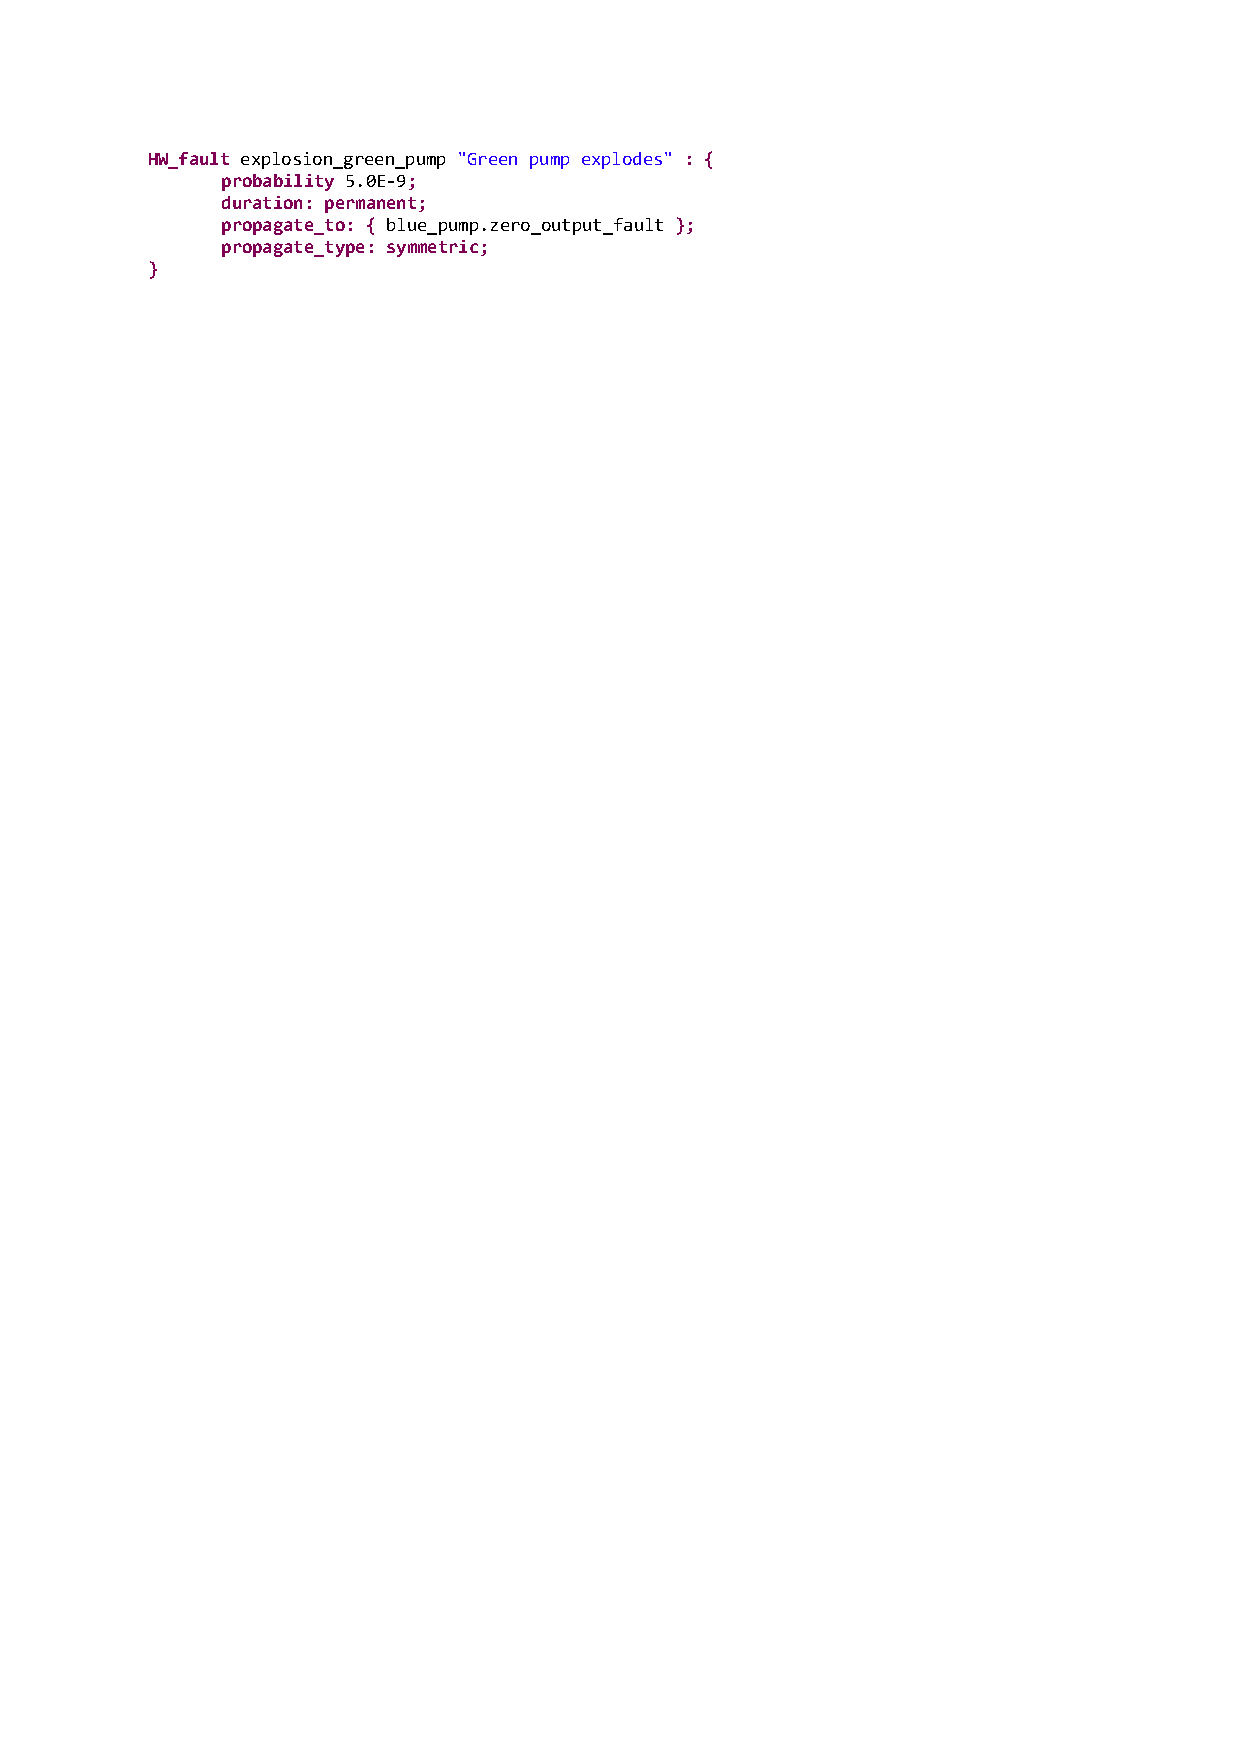
\includegraphics[trim=0 690 -10 70,clip,width=1.5\dimexpr\textwidth-2cm\relax]{images/hw_fault_green_pump.pdf}
		\caption{Hardware fault for the green pump}
		\label{fig:hwFault}
	\end{center}
	\vspace{-0.3in}
\end{figure}

As an example, we will look yet again at the WBS. Assume that both the green and blue hydraulic pumps are located in the same compartment in the aircraft. This particular aircraft was in flight when the zombie apocolypse began and unfortunately a few of the passengers were among the undead. The description of the chaos leading up to the pump compartment accident is unnecessary in order to illustrate hardware fault modeling. It is sufficient to say that due to this series of events, an explosion took place in said compartment. The green (normal) hydraulic pump took the force of the explosion and when the green hydraulic pump exploded, the pump shrapnel flew into the blue (alternate) pump and it became from then on unoperable. 

The HW fault definition can be modeled first in the green hydraulic pump component as shown in Figure~\ref{fig:hwFault}. The activation of this fault triggers the activation of related faults as seen in the \textit{propagate\_to} statement. Notice that these pumps need not be connected through a data port in order to specify this propagation, they need only to be located in the same area of the aircraft. Furthermore, the probability of occurance can be given. This specifies the probability of the HW fault activation. If this HW fault is activated, the probability of propagation is 100\%. (Note: This value in this example does not reflect the probability of a zombie apocolypse, but rather some unforseen event leading to the destruction of the pumps, i.e. fire, water damage, explosion, bullet, etc.)  

\danielle{Danielle comment: I still need to actually define this fault in the WBS system in order to talk about the effects on the system.}
















